\documentclass{article}
\usepackage{comment}
\includecomment{vfull}
\excludecomment{vcat}

\usepackage[margin=1in]{geometry}
\usepackage{mathtools} %also loads amsmath
\usepackage{amssymb, bbm}

\usepackage[backend=biber,
	style=alphabetic,
	%	citestyle=authoryear,
	natbib=true,
	url=true, 
	doi=true]{biblatex}

%\usepackage{blkarray} % for matrices with labels
\usepackage{microtype}
\usepackage{relsize}
\usepackage{environ}% http://ctan.org/pkg/environ; for capturing body as a parameter for idxmats
\usepackage{tikz}
	\usetikzlibrary{positioning,fit,calc, decorations, arrows, shapes, shapes.geometric}
	\usetikzlibrary{cd}
	
	\pgfdeclaredecoration{arrows}{draw}{
		\state{draw}[width=\pgfdecoratedinputsegmentlength]{%
			\path [every arrow subpath/.try] \pgfextra{%
				\pgfpathmoveto{\pgfpointdecoratedinputsegmentfirst}%
				\pgfpathlineto{\pgfpointdecoratedinputsegmentlast}%
			};
	}}
	%%%%%%%%%%%%
	\tikzset{center base/.style={baseline={([yshift=-.8ex]current bounding box.center)}}}
	
	\tikzset{dpadded/.style={rounded corners=2, inner sep=0.9em, draw, outer sep=0.4em, fill=gray, fill opacity=0.08, text opacity=1}}
	\tikzset{active/.style={fill=blue, fill opacity=0.1}}
	\tikzset{square/.style={regular polygon,regular polygon sides=4, rounded corners = 0}}
	\tikzset{octagon/.style={regular polygon,regular polygon sides=8, rounded corners = 0}}
	
	
	\tikzset{alternative/.style args={#1|#2|#3}{name=#1, circle, fill, inner sep=1pt,label={[name={lab-#1},gray!30!black]#3:\scriptsize #2}} }
	
	
	\tikzset{bpt/.style args={#1|#2}{alternative={#1|#2|above}} }
	\tikzset{tpt/.style args={#1|#2}{alternative={#1|#2|below}} }
	\tikzset{lpt/.style args={#1|#2}{alternative={#1|#2|left}} }
	\tikzset{rpt/.style args={#1|#2}{alternative={#1|#2|right}} }
	\tikzset{pt/.style args={#1}{alternative={#1|#1|above}} }
	

	\tikzset{mpt/.style args={#1|#2}{name=#1, circle, fill, inner sep=1pt,label={[name={lab-#1},gray]\scriptsize #2}} }
	\tikzset{pt/.style args={#1}{name=#1, circle, fill, inner sep=1pt,label={[name={lab-#1},gray]\scriptsize #1}} }
	
		
		 %\foreach \x in {#1}{(\x) (lab-\x) } 
		 
	\tikzset{Dom/.style args={#1 (#2) around #3}{dpadded, name=#2, label={[name={lab-#2},align=center] #1}, fit={ #3 } }}
	\tikzset{bDom/.style args={#1 (#2) around #3}{dpadded, name=#2, label={[name={lab-#2},align=center]below:#1}, fit={ #3 } }}
	\tikzset{arr/.style={draw, ->, thick, shorten <=3pt, shorten >=3pt}}
	\tikzset{archain/.style args={#1}{arr, every arrow subpath/.style={draw,arr, #1}, decoration=arrows, decorate}}
	%\tikzset{every label/.append style={text=red, font=\scriptsize}}
	\tikzset{dpad/.style args={#1}{every matrix/.append style={nodes={dpadded, #1}}}}
	\tikzset{light pad/.style={outer sep=0.2em, inner sep=0.5em, draw=gray!50}}
	
	
	\newcommand\cmergearr[4]{
		\draw[arr,-] (#1) -- (#4) -- (#2);
		\draw[arr, shorten <=0] (#4) -- (#3);
	}
	\newcommand\mergearr[3]{
		\coordinate (center-#1#2#3) at (barycentric cs:#1=1,#2=1,#3=1.2);
		\cmergearr{#1}{#2}{#3}{center-#1#2#3}
	}

\NewEnviron{ctikzpicture}{\begin{center}\expandafter\begin{tikzpicture}\BODY\end{tikzpicture}\end{center}}
%\newenvironment{ctikzpicture}
%	{\begin{center}\begin{tikzpicture}}
%	{\end{tikzpicture}\end{center}}

\usepackage{color}
\definecolor{deepgreen}{rgb}{0,0.5,0}

\usepackage[colorlinks=true, citecolor=deepgreen]{hyperref}


\setlength{\skip\footins}{1cm}
\setlength{\footnotesep}{0.4cm}


\usepackage{stmaryrd}
\usepackage{trimclip}

\makeatletter
\DeclareRobustCommand{\shortto}{%
	\mathrel{\mathpalette\short@to\relax}%
}

\newcommand{\short@to}[2]{%
	\mkern2mu
	\clipbox{{.5\width} 0 0 0}{$\m@th#1\vphantom{+}{\shortrightarrow}$}%
}
\makeatother

\usepackage{parskip}
\usepackage{amsthm, thmtools}
\usepackage{
	nameref,%\nameref
	hyperref,%\autoref
	% n.b. \Autoref is defined by thmtools
	cleveref,% \cref
	% n.b. cleveref after! hyperref
}

\hypersetup{colorlinks=true, linkcolor=blue, urlcolor=magenta}

\begingroup
\makeatletter
\@for\theoremstyle:=definition,remark,plain\do{%
	\expandafter\g@addto@macro\csname th@\theoremstyle\endcsname{%
		\addtolength\thm@preskip\parskip
	}%
}
\endgroup
\makeatother

\theoremstyle{plain}
\newtheorem{theorem}{Theorem}[section]
\newtheorem{coro}{Corollary}[theorem]
\newtheorem{prop}[theorem]{Proposition}
\newtheorem{lemma}[theorem]{Lemma}
\newtheorem{fact}[theorem]{Fact}
\newtheorem{conj}[theorem]{Conjecture}

\theoremstyle{definition}
\newtheorem{defn}{Definition}[section]
\newtheorem*{defn*}{Definition}
\newtheorem{examplex}{Example}[section]
\newenvironment{example}
	{\pushQED{\qed}\renewcommand{\qedsymbol}{$\triangle$}\examplex}
	{\popQED\endexamplex\vspace{-1em}\rule{1cm}{0.7pt}\vspace{0.5em}}

\theoremstyle{remark}
\newtheorem*{remark}{Remark}

\usepackage{xstring}
\usepackage{enumitem}

\DeclarePairedDelimiterX{\infdivx}[2]{(}{)}{%
	#1\;\delimsize\|\;#2%
}
\newcommand{\kldiv}{D_\mathrm{KL}\infdivx}
%\DeclarePairedDelimiter{\norm}{\lVert}{\rVert}

%\newcommand\duplicat[1]{\gdef\mylist{}\foreach \x in {#1}{\xdef\mylist{\mylist (\x) (lab-\x) }}\mylist} %% this doesn't work :((
\newcommand\lab[1]{(#1)(lab-#1)}


\newcommand{\CI}{\mathrel{\perp\mspace{-10mu}\perp}}
\newcommand\E{{\mathbb E}}


\newcommand{\todo}[1]{{\color{red}\large\textbf{[}{\normalsize\texttt{todo:} \itshape#1}\textbf{]}}}
\newcommand{\note}[1]{{\color{blue}\large\textbf{[}{\normalsize\texttt{note:} \itshape#1}\textbf{]}}}

\newcommand\geqc{\succcurlyeq}
\newcommand\leqc{\preccurlyeq}
\newcommand\mat[1]{\mathbf #1}
\newcommand{\indi}[1]{\mathbbm{1}_{\left[\vphantom{\big[}#1 \vphantom{\big]}\right]}}
\newcommand\m[1]{\mathbf m_{\mathsf #1}}
\def\cpm#1(#2|#3){\mathbf #1 \left[ #2 \middle|#3\right]}


\newcommand\recall[1]{\expandarg\cref{#1}:\vspace{-1em} \begingroup\small\color{gray!80!black}\begin{quotation} \expandafter\csname #1\endcsname* \end{quotation}\endgroup }

%OMG THIS WORKS

\def\wrapwith#1[#2;#3]{
	\expandafter#2{\expandarg\StrBefore{#1}{,}}
	\expandarg\StrBehind{#1}{,}[\tmp] 
	\xdef\tmp{\expandafter\unexpanded\expandafter{\tmp}}
	#3
	\expandarg\IfSubStr{\tmp}{,}{\wrapwith{\tmp}[#2;{#3}]}{ \expandafter#2{\tmp} }
}
\def\hwrapcells#1[#2]{\wrapwith#1[#2;&]}
\def\vwrapcells#1[#2]{\wrapwith#1[#2;\\]}



\newsavebox{\idxmatsavebox}
\def\makeinvisibleidxstyle#1#2{\phantom{\hbox{#1#2}}}
\newenvironment{idxmatphant}[4][\footnotesize\color{gray}\text]{%
	\def\idxstyle{#1}
	\def\colitems{#3}
	\def\rowitems{#2}
	\def\phantitems{#4}
	\begin{lrbox}{\idxmatsavebox}$
	\begin{matrix}  \begin{matrix} \hwrapcells{\colitems}[\idxstyle]  \end{matrix} \\[0.1em]
		\left[ 
		\begin{matrix}
			\hwrapcells{\phantitems}[\expandafter\makeinvisibleidxstyle\idxstyle]  \\[-1em]
	}{
		\end{matrix}\right]		&\hspace{-0.5em}\begin{matrix*}[l] \vwrapcells{\rowitems}[\idxstyle] \end{matrix*}
	\end{matrix}
	$\end{lrbox}
	\raisebox{0.75em}{\usebox\idxmatsavebox}
%	\vspace{-0.5em}
}

\newenvironment{idxmat}[3][\footnotesize\color{gray}\text]
	{\begingroup\idxmatphant[#1]{#2}{#3}{#3}}
	{\endidxmatphant\endgroup}

\newenvironment{sqidxmat}[2][\footnotesize\color{gray}\text]
	{\begingroup\idxmat[#1]{#2}{#2}}
	{\endidxmat\endgroup}
	
	
%%%%%%%%%%%%
% better alignment for cases
\makeatletter
\renewenvironment{cases}[1][l]{\matrix@check\cases\env@cases{#1}}{\endarray\right.}
\def\env@cases#1{%
	\let\@ifnextchar\new@ifnextchar
	\left\lbrace\def\arraystretch{1.2}%
	\array{@{}#1@{\quad}l@{}}}
\makeatother
\usetikzlibrary{external}
\tikzexternalize[prefix=tikz/]  % activate!

\AtBeginEnvironment{tikzcd}{\tikzexternaldisable} %... except careful of tikzcd...
\AtEndEnvironment{tikzcd}{\tikzexternalenable}



\usepackage[nointegrals]{ wasysym }

\addbibresource{../refs.bib}
\addbibresource{../maths.bib}


% symbols for genders, hour glass.
\newcommand{\mfem}{\mathclap\female\male}
\newsavebox{\hourglassbox}
\savebox{\hourglassbox}{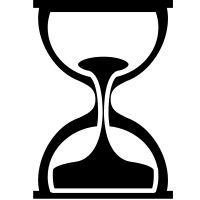
\includegraphics[height=.8em]{hourglass.png}}
\newcommand\hourglass{\usebox{\hourglassbox}}

\newcommand{\modelname}{Probabilistic Dependency Graph}
\newcommand{\modelnames}{Probabilistic Dependency Graphs}
\newcommand{\MN}{PDG}
\newcommand{\MNs}{PDGs}

\title{Dependency Graphs}
\author{Oliver Richardson,  \texttt{oli@cs.cornell.edu}}

\begin{document}
	\maketitle
	
	\begin{abstract}
		We introduce \modelnames, intended to represent agents' mental states, which can be regarded both as a probabilistic graphical model, and as a collection of soft, local, constraints. The additional representational flexibility allows us to represent both under and over-constrained belief states, as well as a modularity that makes the models easier to modify. They are also easier to use, have a clean theoretical backing, and reduce appropriately to existing, commonly used representations such as Bayesian Networks and constraint graphs. Some algorithms, notably including belief propagation, lift to the more general setting.
	\end{abstract}
	
	\section{Introduction}
%	Because writing down distributions explicitly is intractable, and so it is necessary to have.
	Inconsistency is bad. Believing a logically inconsistent formula can lead you to arbitrarily bad conclusions, having an infeasible set of constraints makes all answers you could give wrong, and having inconsistent preferences can make you infinite money. We don't want to build inconsistent systems with undefined behavior, and so we design them so they cannot possibly be inconsistent. For example, is unwise to parameterize a unit circle with an $x$ and $y$ coordinate, because $x^2+ y^2$ might not be 1 --- it would be safer and harder to go awry if we parameterize it by an angle $\theta \in [0, 2\pi)$ instead. Why would we take the first approach, introducing a potentially complex data-invariant, when we could avoid it?
	
	This line of thought, though common and defensible, is flawed if we are not perfectly confident in the design of both our system and the ways it can interact with the outside world. Using similar logic, we might ask ourselves: Why ask programmers for type annotations when all operations are well-defined at run-time?  Why use extra training data if there's already enough there to specify a function? Why estimate a quantity in two ways when they will yield different answers? Why repeat and rephrase your ideas when this could make you contradict yourself? Why write test cases when they could fail and make the project inconsistent? Why conduct an experiment if it could just end up contradicting everything you know?
	
	These questions may seem silly, but there is a satisfying information theoretic answer to all of them: redundancy, though costly, is the primary tool that we use to combat the possibility of being wrong. Maintaining data invariant is expensive but provides diagnostic information; in the example above, settings of $x$ and $y$ that don't lie on the unit circle provide diagnostic information that some part of your algorithm is broken. In many cases, it is also possible to paper over problems by forcibly re-instating local data invariants: for instance, we could re-normalize any values of $x$ and $y$ (so long as $xy \neq 0$; we can chose an arbitrary point otherwise) at every step. While this would reduce inconsistency, it also hides red flags. 
	
	Using a Bayesian Network is like representing a circle with $\theta \in [0, 2\pi)$. By construction, the result must be a point on the circle, and nothing can possibly go wrong so long as we're sure that we will always have exactly enough information to determine such a point (for instance, we could never not know the point, or just know its $x$ coordinate). 
	The process of mechanistically forcing invariants is exactly homologous to standard practices for factor graphs (or Gibbs Random Fields): practitioners will often just assume that the density it defines is normalizable, and either forcibly re-normalize or cleverly avoid computing the normalization constant while still assuming that one exists; behavior is usually left unspecified in the unlikely event that it is not defined or zero. 
	
	It is clear that, while inconsistency is bad, being able to identify it is extremely useful. To that end, we introduce a more general representation which can be both under and over-constrained (from the perspective of producing a probability distribution), can be used to emulate a large class of both probabilistic models and constraint sets, and enjoys many additional properties which make them more useful than the specific variants. All of this comes at the cost of being slightly more difficult to analyze in general case: most decision problems on \modelnames\ are NP hard. % and some are incomputable. 
	
	
	\begin{example}
		Suppose we have a belief about how size and composition affect the habitability of a planet: say we're astrobiologists, and for mechanistic reasons, we know how likely you are to find life on a planet, supposing we knew how big it is, and whether it's mostly made of rocks or gas. We have a conditional density $\Pr(\text{Life} ~|~ \text{Size}, \text{Composition})$, which we would like to represented as a Bayesian network
		\begin{ctikzpicture}
			\node[dpadded] (SS) at (0, 2) {Size};
			\node[dpadded] (CC) at (3, 2) {Composition};
			\node[dpadded] (LL) at (1.3,0) {Life};
			\draw[arr] (CC) -- (LL);
			\draw[arr] (SS) -- (LL);
		\end{ctikzpicture}
		but this is technically incorrect because a BN would require that we also have prior distributions over both the size of planets and their compositions. Our actual mechanistic knowledge is under-constrained in this picture. But to be good Bayesians, we also need priors on everything, which is unfortunate, but we can always make one up and refine it as we go along. A bigger problem occurs when our biologist friend reminds us that life requires water, and gives us a probability estimate for the existence of life on a planet, with and without water. We trust this friend, and totally believe these probabilities, but there's no way to incorporate it into our picture, because we don't know what the correlations are between water, size, and composition; neither are we prepared to give a probability of live given a full description of the three, and we don't even have the space to keep such a thing. At this point the Bayesian Network is not at all a convenient way of storing the information at hand.
		
		Instead, we want a picture that looks more like this:
	
	
		\begin{ctikzpicture}
			\node[dpadded] (S) at (0, 2) {Size};
			\node[dpadded] (C) at (3, 2) {Composition};
			\node[dpadded] (L) at (1.3,0) {Life};
			\node[dpadded] (W) at (-2,0) {Water};
			\mergearr{S}{C}{L}
			\draw[arr] (W) -- (L);
		\end{ctikzpicture}
		which allows us to combine our knowledge, even though there's a possibility of being inconsistent --- for instance, if all estimates of the probability of life from the existence of water are strictly smaller than the estimates we initially came up with.
	\end{example}

	Benefits of this representation:
	\begin{enumerate}[nosep]
		\item We can represent both over-constrained and under-constrained mental states, both of which we argue are an important component of an agent's state.
		\item Over-constrained models may be inconsistent; such inconsistencies provide a natural way of prescribing changes in mental state. Moreover, many standard algorithms, such as belief updating via Jeffrey's rule, as well as marginalization algorithms such as belief propagation, can be regarded as special cases of consistency reduction.
		\item We can emulate both other graphical models (such as Bayesian Networks, and to a large extent, factor graphs), as well as other non-probabilistic notions of uncertainty. 
		\item The local interpretation of arrows makes it much less invasive to add, remove, and partially interpret parts of the model, compared to other graphical models. 
		\item This modularity makes it possible to add explicit rules to embed logic within the model
		\item By allowing agents to merge, split, and compress variables, we also make it possible for agents to design their own representations. With these tools, in conjunction with consistency 
		\item In contrast with a simple collection of constraints, inconsistencies are local, and individual mistakes have limited impact on expectations.
	\end{enumerate} % trade-off: harder to analyze.


%	\begin{enumerate}[nosep]
%		\item This representation more naturally matches what humans are aware of, encoding small locally consistent models rather than one giant probability distribution
%		\item It is a strictly more general representation--- we can easily convert BNs to these diagrams (section \ref{sec:convert2bn})
%		\item This allows composition of arrows to be defined, and gives meanings to paths (section \ref{sec:composition}).
%		\item Allowing variables to be added and removed makes 
%		\item Changing and partially determining arrows is more reasonable.
%		\item We can now represent inconsistency, which will allow us to capture mental states which, and . While we agree with the classical picture in that inconsistency is bad, now we can talk about it
%	\end{enumerate}
	
	
	% Redundency is important: types in programming languages, more data in ML systems. 
	% Puts gurads
	% Makes it possible to combine knowledge without destroying old knowledge.
	% preference updating
	\section{Related Work}
	
	\section{Worlds}
	Other than allowing for inconsistency, the biggest difference between \modelnames and other graphical models is their interaction with the underlying space: a \modelname . The standard approach to probabilistic modeling is to start by selecting a measurable space of possible outcomes $\Omega$, and then put a normalized measure on it and compute desired quantities with it. Before you can begin to think about random variables, which are defined as set $X_i : \Omega \to V_i$ from outcomes to the set of values $V_i$ that $X_i$ can take on, you have to specify $\Omega$. This construction works well, so long as $\Omega$ is large enough to express everything you ever cared to conceptualize. Because agents are expected to have probability distributions over $\Omega$, the set of worlds that they consider possible must effectively stay constant over time, to use mechanisms such as conditioning as a sole way of changing a mental state. 
	
	Still, a we might wiggle our way around this using only classical probability: we could say that $\Omega$ is some very large set of outcomes that is guaranteed to be expressive enough to capture anything we care about, and then 
	
	To be clear, we've already given up on the possibility of being a Bayesian, because we clearly don't have priors on arbitrary concepts we haven't considered yet if we don't even know the extent of the space, but we might be able to do this with some under-constrained mechanism. 
	
	This strategy, works so long as you are an omniscient modeler. If you are modeling a system in which you know the set of all possible outcomes, either implicitly or explicitly, you can just collect them and use this to be $\Omega$, marginalize out appropriately, and let agents figure out their own distributions on subspaces of $\Omega$. Still, this is not entirely satisfying, for several reasons. 
	
	
	\todo{most of these are unfinished thoughts, some need to be deleted}
	\begin{enumerate}
		\item While it is true that the there will be subspaces of $\Omega$ which are isomorphic to the sets of worlds $W_i$ that the agents are modeling in their heads, the embedding is not at all clear \todo{}
		
		\item There may not be an omniscient modeler, and even if there were one, it seems very strange for an agent to have any access to it. Suppose you are using probabilities to describe real uncertainties in your life. To do this the standard way, you need to chose the subspace of the one true $\Omega$ \todo{why is this problematic? for reasons other than inability to change?}
		
		\item Agents can never gain access via any standard mechanism to new worlds. There's no principled way to add worlds from $\Omega$ to $W_i$. Effectively, they can never learn new concepts.
		
		\item Any updates must be done on the entire space of things you consider possible \todo{response: of course, this is all handled implicitly, so it's taken care of}.
		
		\item While agents are free to merge multiple states of $\Omega$ into a single state in $W_i$, they cannot do the reverse: an agent cannot have a finer granularity than $\Omega$ for discerning events. This would . This also implies that agents are logically omniscient.
	\end{enumerate}

	For all of these reasons, we take the view that probability should be thought of subjectively, 
	
%	\footnote{in addition to being notoriously counter-intuitive.}
	
	At the same time, starting with a set of random variables $\{X_i\}$, and setting $\Omega = \prod_{i} V_i$ to be every possible assignment of variables is also an abuse of the word ``possible''.
	
	
	\section{Definitions and Semantics}
	
	
	
	\begin{defn}
		A \emph\modelname\ is 
	\end{defn}
	
	
	\subsection{Sub-stochastic Transitions}
	
	\subsection{Semantics}
	These graphs admit multiple semantics. As discussed in section \ref{sec:worlds}, we think of \modelnames\ as being a representation of knowledge in and of themselves, rather than a compression of something more fundamental such as a probability distribution. Still, we will find it useful to interpret them in various ways: doing so will make it possible to compare them more directly with existing graphical models, which one thinks of as really just being compressed distributions. In this section, we would like to highlight three important semantics. 
	
	\subsubsection{As Distributions}
	
	\section{Rebuilding Probability}
	
	\section{Relations to Other Graphical Models}
	\subsection{Bayesian Networks}
	\subsection{Factor Graphs}
	
	\section{Relations to Other Representations of Uncertainty}
	\modelnames\ are far from the first formalism to provide a weaker notion of uncertainty than probability. Belief functions, inner measures, sets of probabilities, lower probabilities, weighted sets of probabilities, and plausibility measures have all been studied extensively in the past. One feature that each of these has in common is that they are under-specified, from the perspective of wanting probabilities for everything. 
	
	The natural question now becomes: to what do these under-constrained representations of belief correspond to under-constrained bits of a \modelname?
	
	\subsection{Sets of Probability Measures}
	As may have been clear 
	
	
	
	\section{Using Inconsistency}
	
	Given a distribution $\mu$, and a 
	
	\section{Algorithms}
	\subsection{Belief Propagation}
	
	\section{Conclusions}
\end{document}